\newcommand{\paramspace}{{\color{MacroColor}\Theta}}
\newcommand{\modelparams}{{\color{MacroColor}\vtheta}}
\newcommand{\model}{{\color{MacroColor}\pM^\vtheta}}
\newcommand{\loglike}{{\color{MacroColor}\mathcal{L}}}
\newcommand{\vthetamle}{{\color{MacroColor}\modelparams{\mathrm{MLE}}}}
\newcommand{\corpus}{{\color{MacroColor}\mathcal{D}}}
\newcommand{\corpustrain}{{\color{MacroColor}\mathcal{D}_{\scaleto{\text{train}}{4pt}}}}
\newcommand{\corpustest}{{\color{MacroColor}\mathcal{D}_{\scaleto{\text{test}}{4pt}}}}
\newcommand{\corpusval}{{\color{MacroColor}\mathcal{D}_{\scaleto{\text{val}}{4pt}}}}
\newcommand{\calX}{{\color{MacroColor}\mathcal{X}}}
\newcommand{\ent}{{\color{MacroColor}\mathrm{H}}}
\newcommand{\objective}{{\color{MacroColor}O}}
\newcommand{\loss}{{\color{MacroColor}\ell}}
\newcommand{\datasize}{{\color{red}N}}
\newcommand{\dataidx}{{\color{red}n}}
\newcommand{\numtimesteps}{{\color{red}T}}
\newcommand{\timeidx}{{\color{red}t}}
\newcommand{\desiderata}{{\color{MacroColor}S}}
\newcommand{\learningrate}{{\color{MacroColor}\boldsymbol\eta}}
\newcommand{\updatedir}{{\color{MacroColor}U}}
\newcommand\bertbase{BERT$_{\textsc{BASE}}$\xspace}
\newcommand\bertlarge{BERT$_{\textsc{LARGE}}$\xspace}

\section{BERT}

After the success of ELMO, \citet{devlin-etal-2019-bert} pre-trained BERT (Bidirectional Encoder Representations from Transformers), a Transformer-based bidirectional masked language model. BERT is pre-trained with the masked language modeling objective on large scale text corpus. After pre-training, BERT can be fine-tuned to perform different NLP task without the need of design task-specific architectures. BERT advanced the state-of-the-art of many NLP benchmarks at the time it was proposed.

In this section, we first introduce the pre-training objective of BERT. We then describe BERT model architecture and the pre-training and fine-tuning paradigm.

\subsection*{BERT Pre-training Objectives}

BERT is pre-trained jointly with two self-supervised tasks: \textbf{masked language modeling} and \textbf{next sentence prediction}.
This is done at the same time.
The losses for each task are computed and summed together:
$$
\mathcal{L} = \mathcal{L}_\text{MLM}+\mathcal{L}_\text{NSP}
$$

\paragraph{Masked Language Modeling.} \index{masked language modelling}
Masked language modeling (MLM) is first proposed by \citet{cloze} in the literature, who referred to this as a Cloze task. \citet{devlin-etal-2019-bert} adapted this task as a novel pre-training task to overcome the drawback of the standard unidirectional LM.In the masked language modeling setup, the goal is to predict the omitted token from a piece of text that constitutes a logical and coherent completion. For example, in the piece of text
''The students \texttt{[MASK]} to learn about language models'', we predict \textit{want} or \textit{like} with high probability for the \texttt{[MASK]} position. The goal of masked language modeling is to approximate the probability distribution over tokens in our vocabulary as the original token at a given masked position. %that can  masked positions. 
Similarly to the standard language modeling objective, we can choose model parameters by optimizing for the log-likelihood of a dataset $\mathcal{D}$. Albeit in this case, the words at a percentage of randomly-chosen positions in $\mathcal{D}$ are replaced with  \texttt{[MASK]} and the model is given \textbf{both} sides of context around the masked token in order to make its prediction: 

\begin{equation}\label{eq:mlm}
    \gL_{\texttt{MLM}}(\modelparams) = \sum_{\dataidx=1}^{\datasize}\sum_{\tstep=1}^\strlen \log\pMLM(\sym_\tstep^{(\dataidx)}\mid \str_{<\tstep}^{(\dataidx)}, \str_{>\tstep}^{(\dataidx)}; \modelparams)\mathbbm{1}\{\sym_\tstep^{(\dataidx)}\! = \! \texttt{[MASK]}\}
\end{equation}

However, this pre-training method will create a mismatch between the pre-training phase and the fine-tuning phase because the mask token does not appear during the fine-tuning phase. Empirically, to deal with this issue, \citet{devlin-etal-2019-bert} used a special \texttt{[MASK]} token 80\% of the time, a random token 10\% of the time and the original token 10\% of the time to perform masking.

\paragraph{Next Sentence Prediction.} \index{next sentence prediction}
The next sentence prediction objective is included to enable the model to capture the relationships between two consecutive sentences. This is important because many NLP tasks require understanding the relationship between different text inputs (e.g., question and context for the question answering task). By pre-training the model to predict whether a given sentence follows another sentence, we can help the model learn the dependencies and relationships between sentences.

\begin{figure*}[t!]
  \centering
    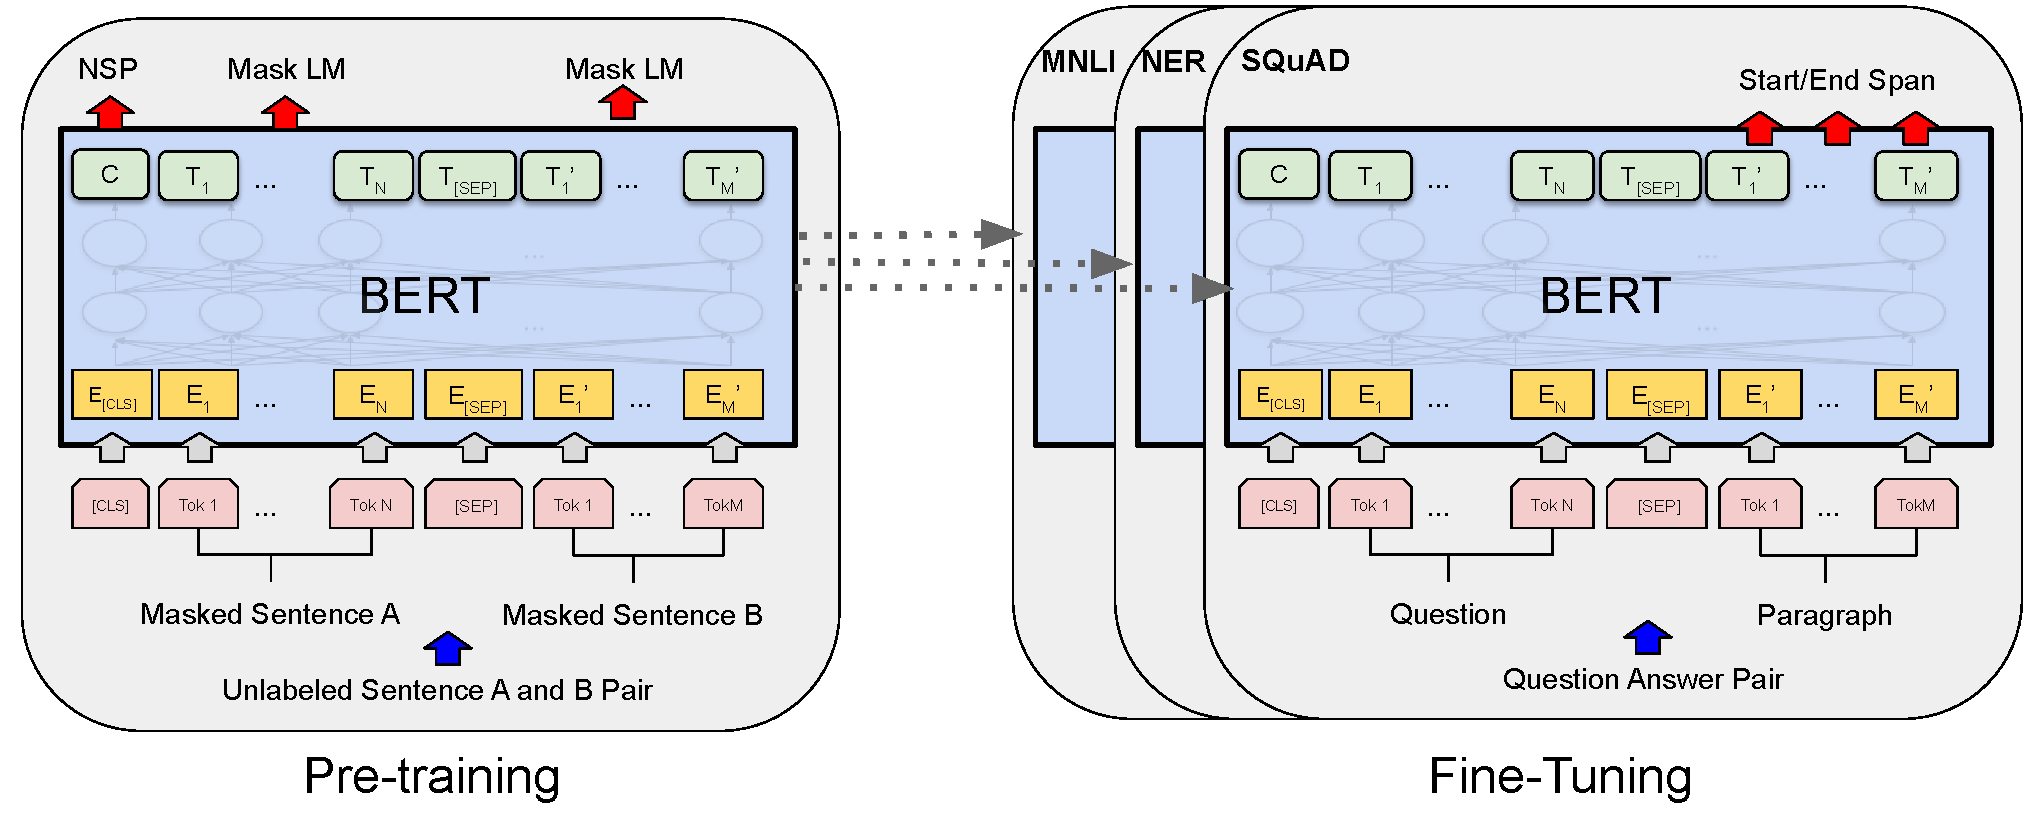
\includegraphics[width=\textwidth]{figures/transfer_learning/BERT_Overall.pdf}
  \caption{Illustration of BERT model architecture.}
  \label{fig:chp3_bert_overall}
  \vspace{-3mm}
\end{figure*}

The next sentence prediction objective is implemented as follows. Given a pair of sentences, denoted as $A$ and $B$, the model is trained to predict whether $B$ is the next sentence that follows $A$. This is done by feeding the two sentences as input to the model, along with a special [CLS] token that serves as the input representation of the entire sequence. The model then generates a binary output that indicates whether $B$ is the next sentence.

BERT is pre-trained with the combination of the masked language modeling objective and the next sentence prediction objective on English Wikipedia data and the BookCorpus~\citep{zhu2015aligning} dataset, which is a collection of over 11,000 books from various genres. The resulting corpus contains over 20 GB of text with over 3.3 billion words and approximately 800 million sentences. BERT is pre-trained with a batch size of 256 sequences for 1M steps.

\subsection*{BERT Architecture}

As illustrated in \Cref{fig:chp3_bert_overall}, BERT's model architecture is a multi-layer bidirectional Transformer encoder. BERT is a Transformer encoder model. It takes a sequence of text tokens as input and produces their contextualized representations and (optionally) predictions. We denote the number of layers (i.e., Transformer blocks) as $L$, the hidden size as $H$, and the number of self-attention heads as $A$.
In all cases the feed-forward/filter size is set to be $4H$, i.e., 3072 for the $H=768$ and 4096 for the $H=1024$.
\citet{devlin-etal-2019-bert} pre-trained two model sizes: {\bf \bertbase} (L=12, H=768, A=12, Total Parameters=110M) and {\bf \bertlarge} (L=24, H=1024, A=16, Total Parameters=340M).


\paragraph{Input/Output Representations.}
To make BERT handle a variety of down-stream tasks,
BERT input representation is able to unambiguously represent both a single sentence and a pair of  sentences (e.g., $\langle$ Question, Answer $\rangle$) in one token sequence. BERT use WordPiece embeddings \cite{wu2016google} with a 30,000 token vocabulary.
The first token of every sequence is always a special classification token ({\tt [CLS]}). The final hidden state corresponding to this token is used as the aggregate sequence representation for classification tasks. Sentence pairs are packed together into a single sequence. We differentiate the sentences in two ways. First, we separate them with a special token ({\tt [SEP]}). Second, we add a learned embedding to every token indicating whether it belongs to sentence {\tt A} or sentence {\tt B}. 
% As shown in Figure~\ref{fig:fi}, we denote 
% input embedding as $E$, the final hidden vector of the special {\tt [CLS]} token as $C \in \mathbb{R}^{H}$, and the final hidden vector for the $i^{\rm th}$ input token as $T_i \in \mathbb{R}^H$.
For a given token, its input representation is constructed by summing the corresponding token, segment, and position embeddings. 
A visualization of this construction can be seen in \Cref{fig:chp3_bert_embedding}.

\begin{figure*}[t!]
  \centering
    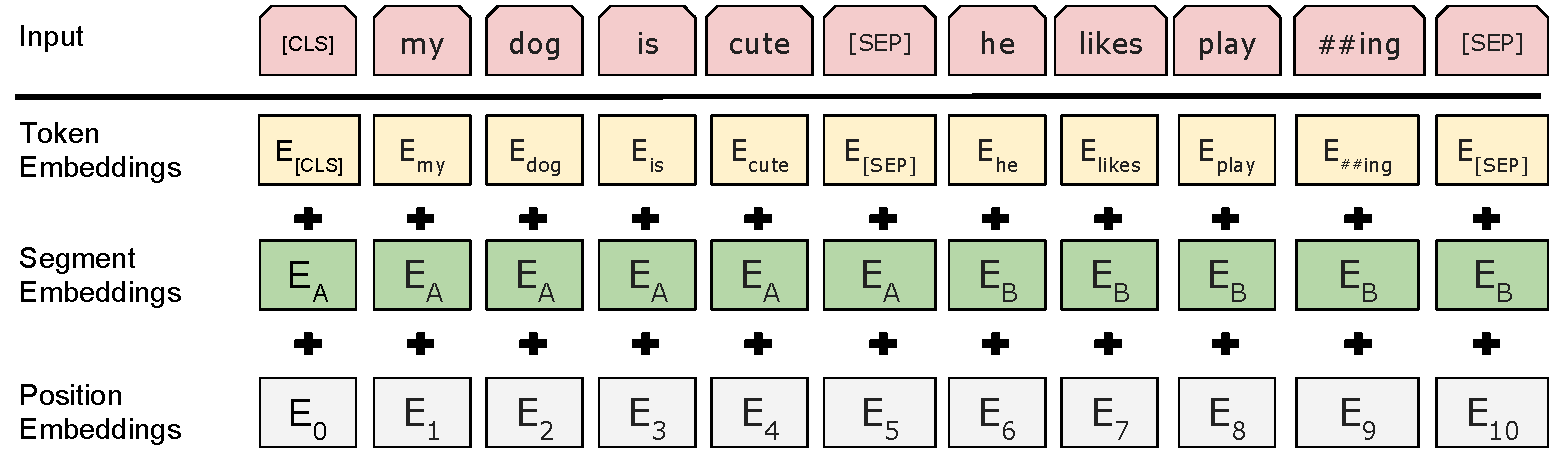
\includegraphics[width=\textwidth]{figures/transfer_learning/Input_Emebeddings.pdf}
  \caption{BERT input representation. The input embedding are the sum of the token embeddings, the segmentation embeddings and the position embeddings.}
  \label{fig:chp3_bert_embedding}
\end{figure*}


\subsection*{BERT Fine-tuning}

\begin{figure*}[t!]
  \centering
    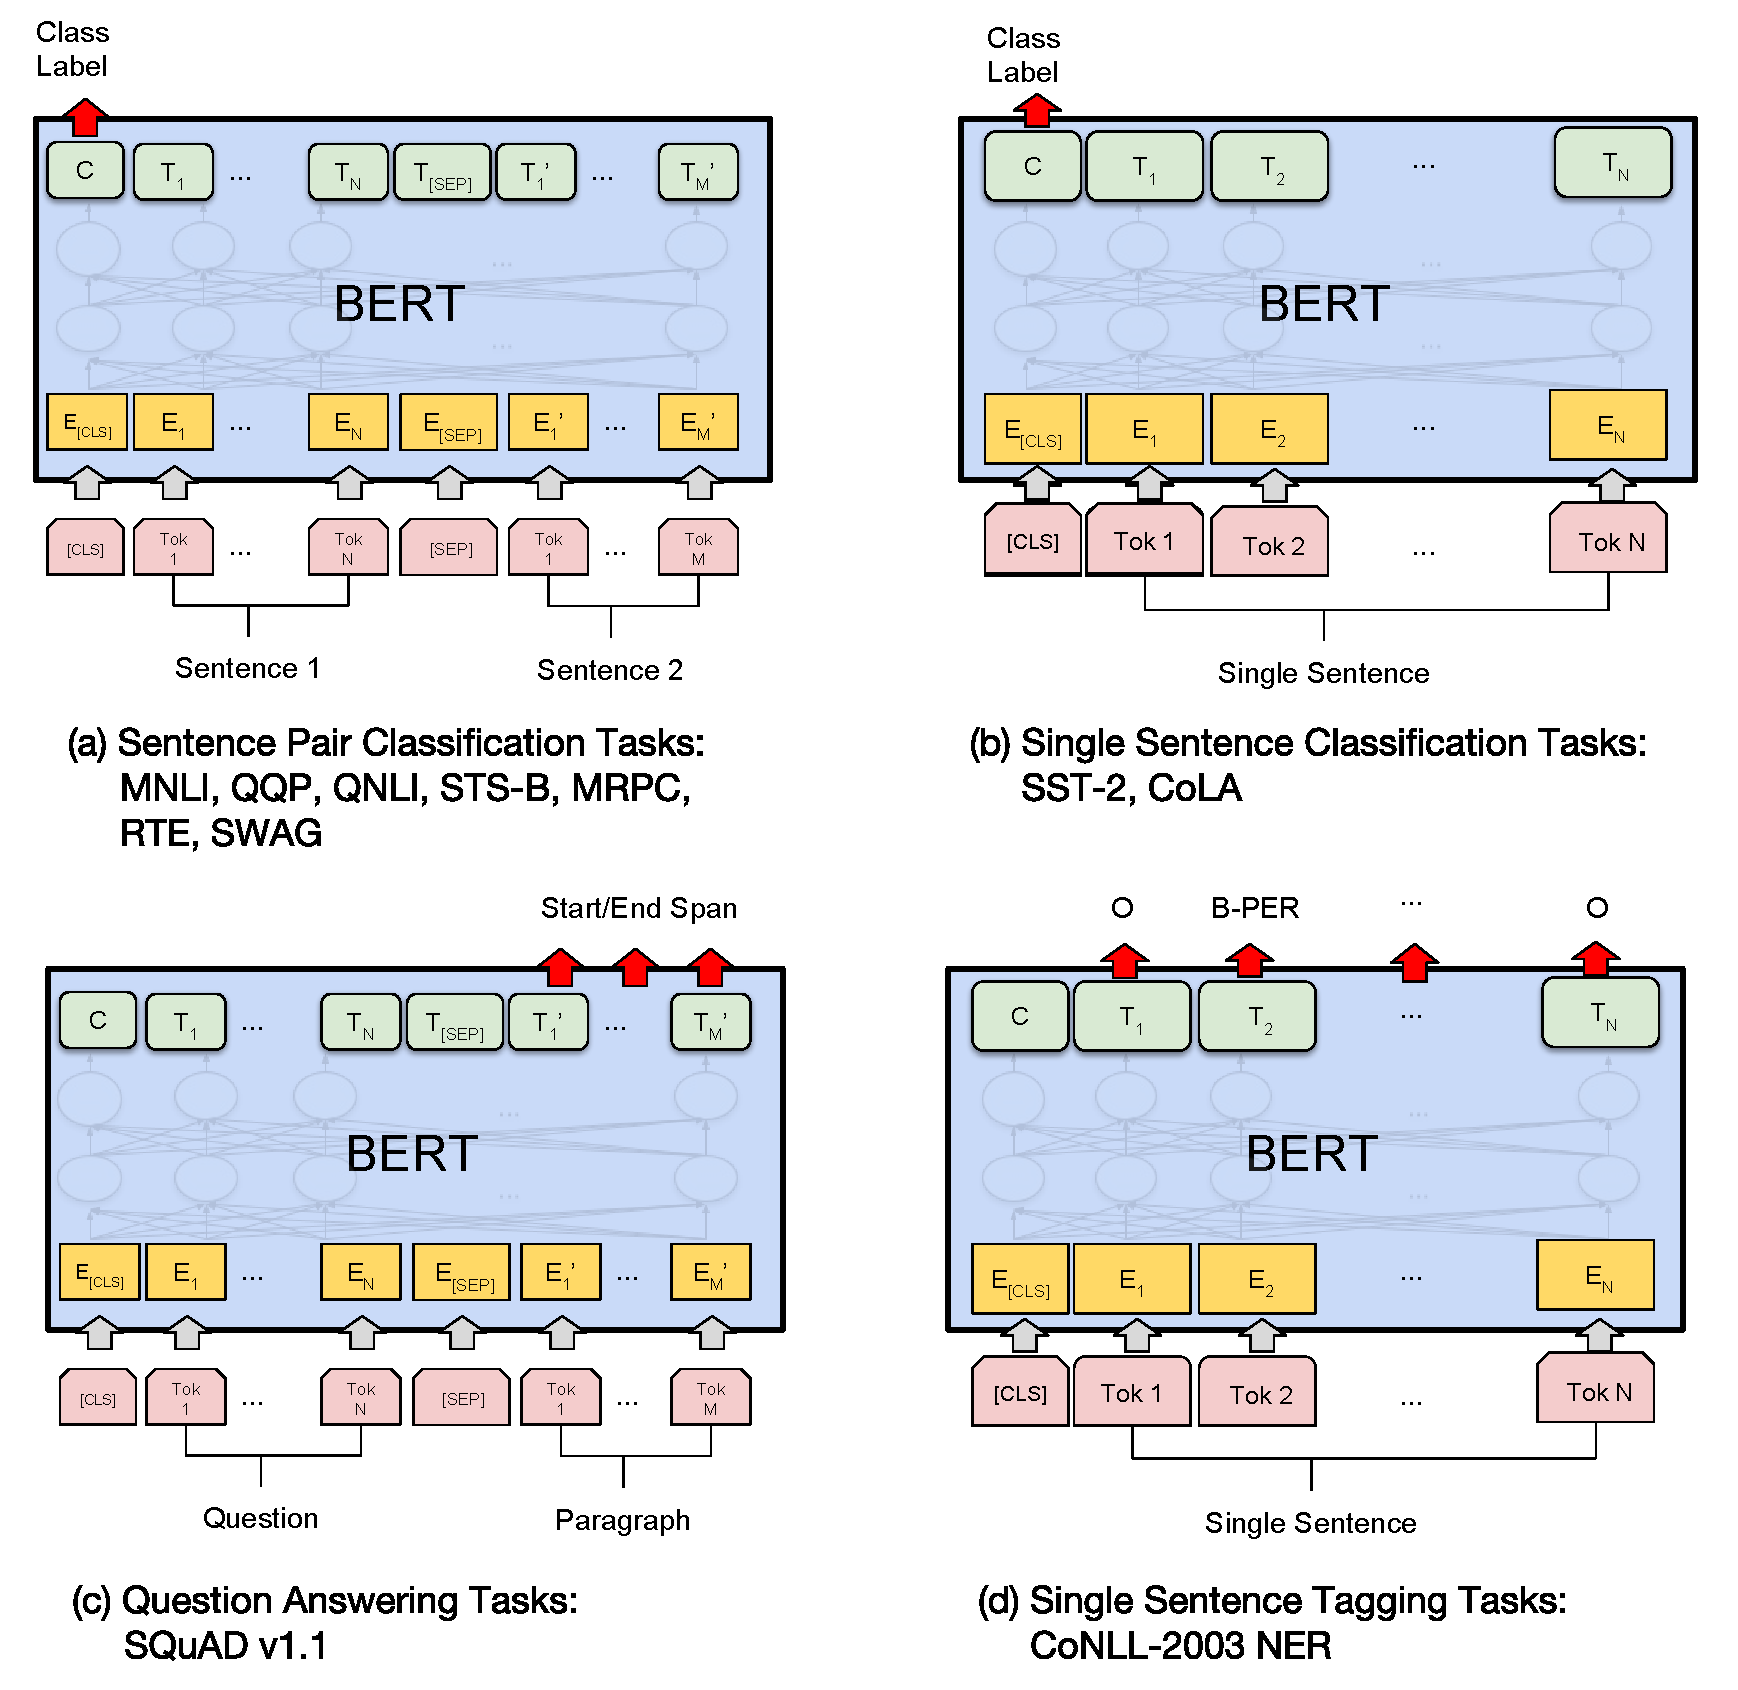
\includegraphics[width=0.9\linewidth]{figures/transfer_learning/BERT_fine_tune.pdf}
  \caption{Illustration of BERT fine-tuning procedure for different NLP tasks.}
  \label{fig:chp3_bert_finetuning}
\end{figure*}

To apply pre-trained BERT models on different downstream tasks, we can simply plug in the task-specific inputs and outputs into BERT and fine-tune all the parameters end-to-end. This \textit{pre-training and fine-tuning} paradigm alleviates need of designing or including any task-specific architectures as EMLO does.

%\mrinmaya{See my slides; we can maybe add some figures from there on finetuning for different tasks and a couple of key results.}



As illustrated in \Cref{fig:chp3_bert_finetuning}, at the input, sentence {\tt A} and sentence {\tt B} from pre-training are analogous to (1) sentence pairs in paraphrasing, (2) hypothesis-premise pairs in entailment, (3) question-passage pairs in question answering, and (4) a degenerate text-$\varnothing$ pair in text classification or sequence tagging. At the output, the token representations are fed into an output layer for token-level tasks, such as sequence tagging or question answering, and the {\tt [CLS]} representation is fed into an output layer for classification, such as entailment or sentiment analysis.
As shown in \Cref{fig:chp3_bert_finetuning_result}, BERT substantially outperforms both ELMo and OpenAI GPT, as well as all previous state-of-the-art on the GLUE benchmark. This confirms the effectiveness of pre-training a bi-directional Transformer encoder using the masked language modeling objective.

\begin{table*}[htbp]
  \centering
    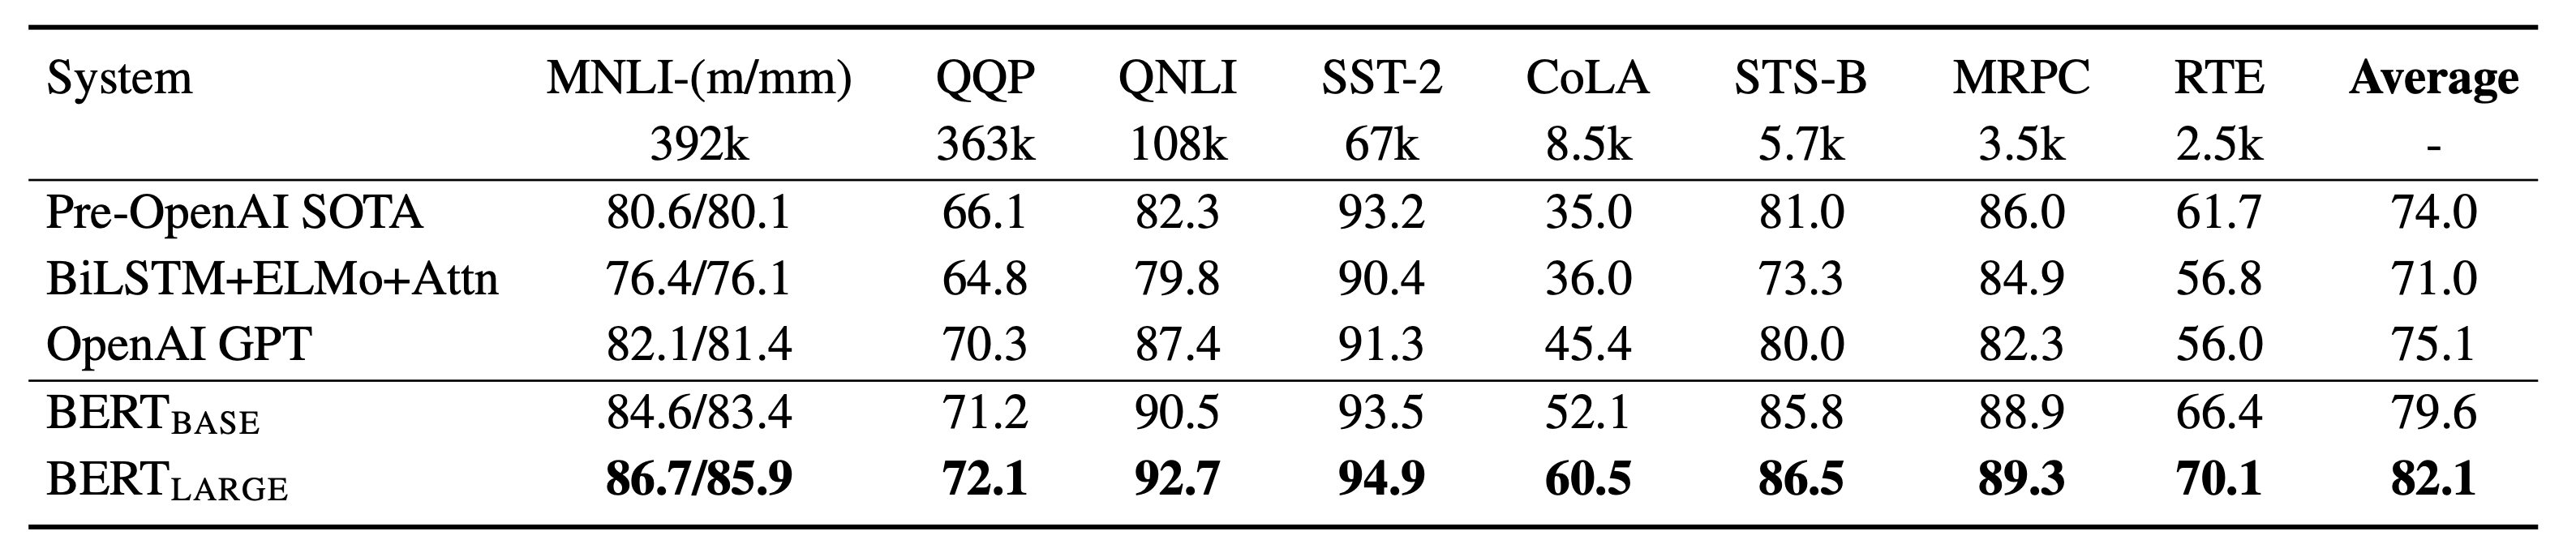
\includegraphics[width=\textwidth]{figures/transfer_learning/bert_results.png}
  \caption{Experimental results of fine-tuning BERT on the GLUE benchmark. }
  % \TODO{Take PDF screenshot instead of PNG}
  \label{fig:chp3_bert_finetuning_result}
\end{table*}

% \section{Other Transformer Language Models}

\section{BERT Variants}

Insipred by the success of BERT, a number of Transformer Language Models (TLMs) have been pre-trained. We categorize these TLMs to three types according to their architecture designs: (i) BERT variants, which are Transformer encoder models, (ii) GPTs, which are Transformer decoder models, and (iii) Seq2Seq TLMs, which are Transformer encoder-decoder models.
After the success of BERT, the community made a lot effort to improve the performance of BERT-like Transformer encoders. We describe a few representative work as follows:

\subsection*{RoBERTa}
RoBERTa (Robustly Optimized BERT Approach) is an optimized version of BERT developed by~\citet{liu2019roberta}. RoBERTa uses the same model architecture of BERT but with some improvements to the pre-training process. RoBERTa uses a larger pre-training corpus, larger batch size, longer training time, longer input sequence lengths, larger batch size, and a dynamic masking strategy during pre-training.
 
Specifically, RoBERTa adds CC-NEWs and OpenWebText to the original BERT pre-training data. The resulting corpus contains over 160 GB of text and approximately 2.5 billion word pieces. RoBERTa is pre-trained with a batch size of 8,000 sequences of 512 tokens for 500k steps, resulting in much more computation compared to BERT. The dynamic masking strategy, which randomizes the masking pattern in each epoch and helps the model to learn more robust representations of the input text. These modifications allows it to surpass BERT and achieve state-of-the-art performance on several NLP tasks at the time.


% \mrinmaya{The caption is confusing. This is only for XLNet I think.}
\begin{figure*}[t!]
  \centering
    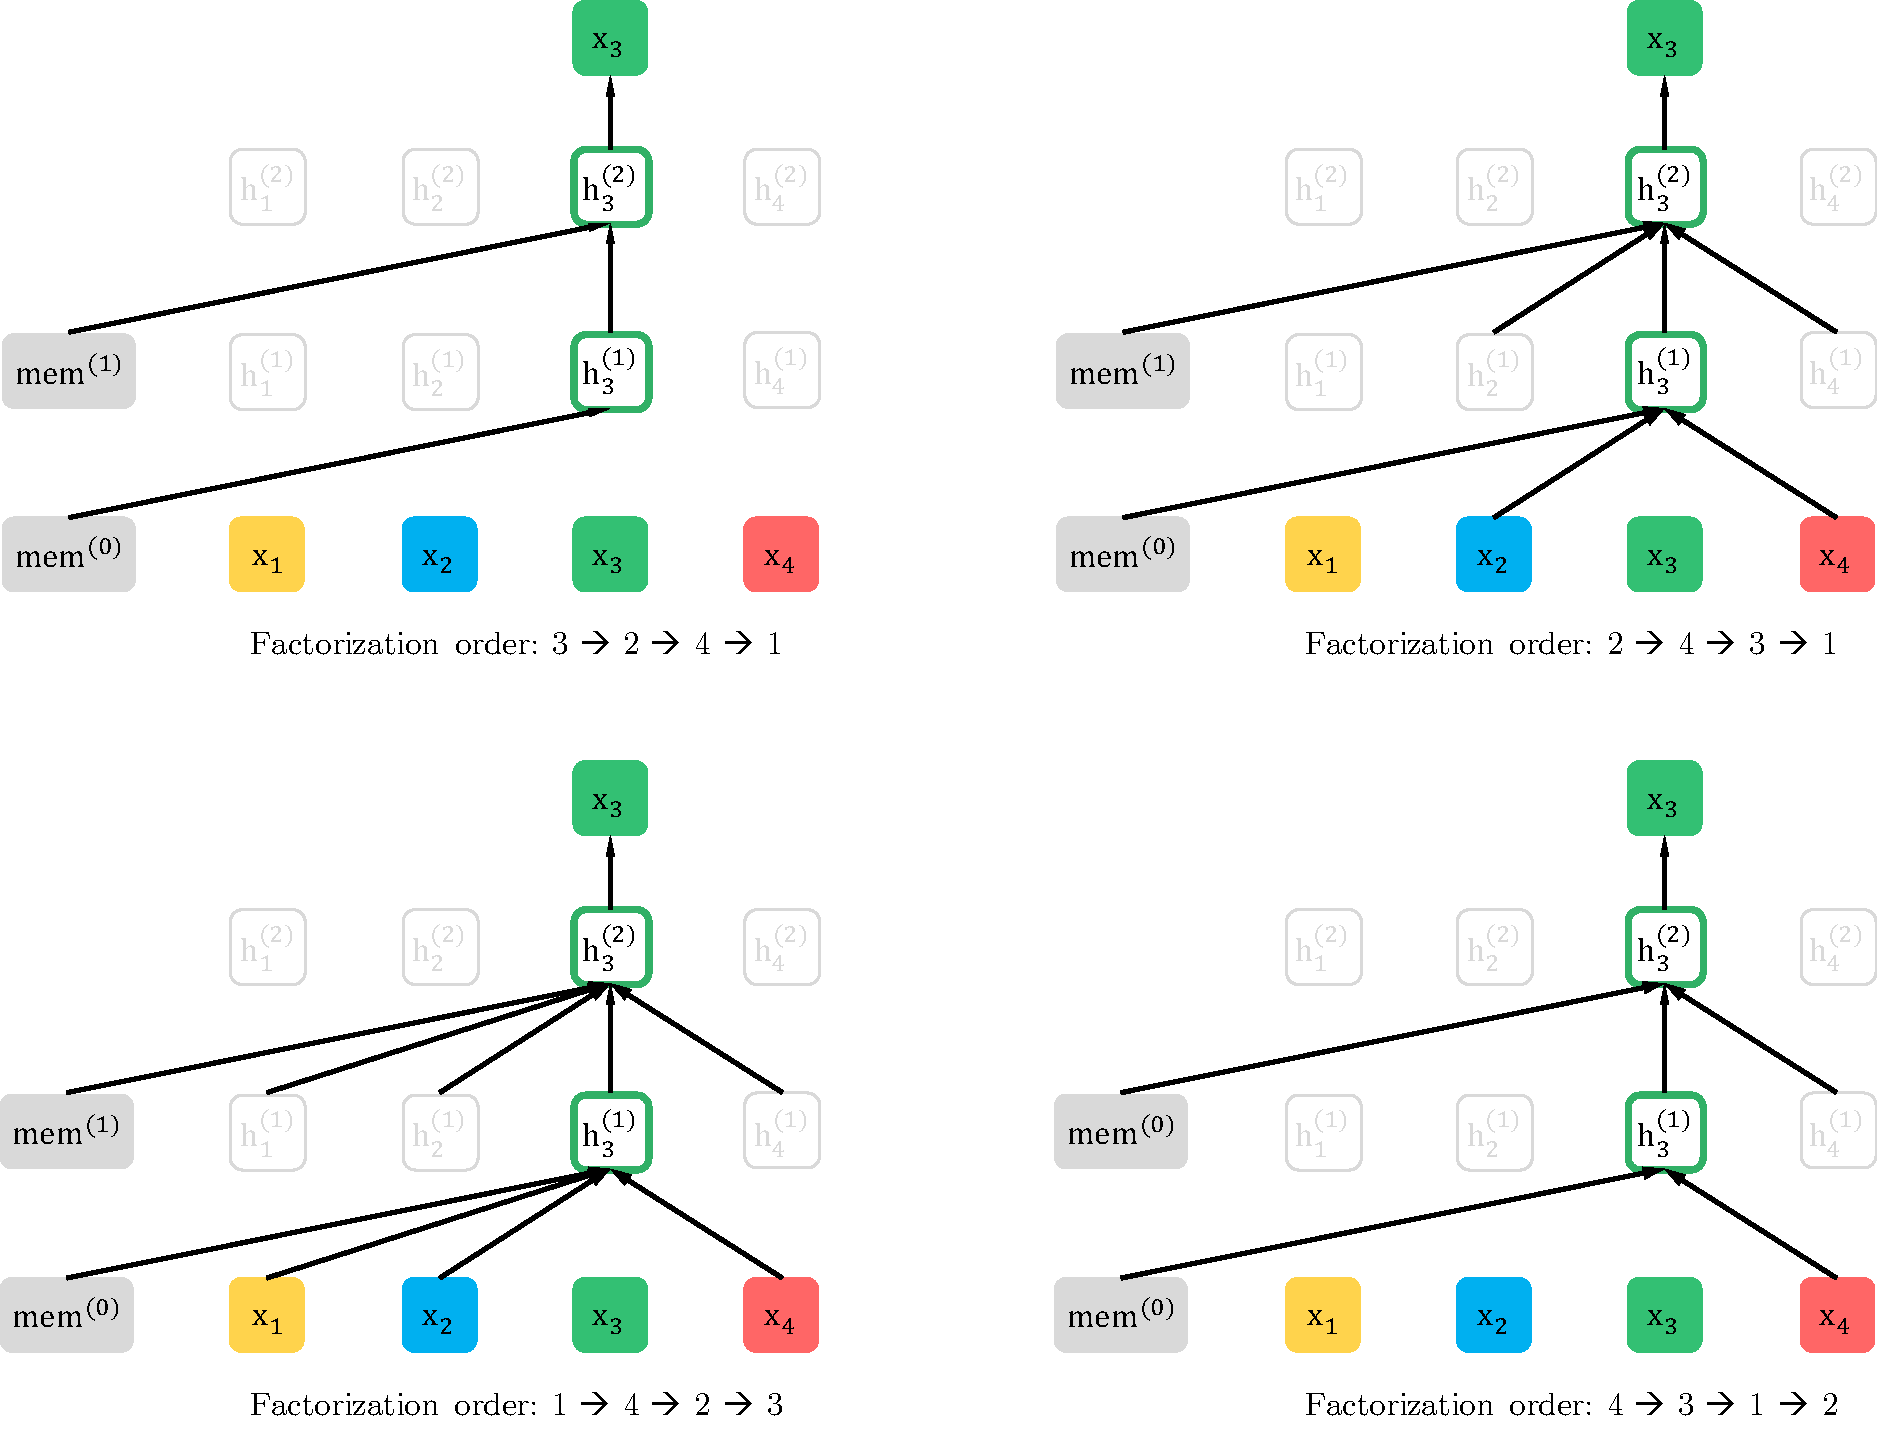
\includegraphics[width=\textwidth]{figures/transfer_learning/fix_pos.pdf}
  \caption{Illustration of the factorization scheme in the permutation language modeling objective of XLNet.}
  \label{fig:xlnet}
\end{figure*}

%\mrinmaya{We can describe the motivation first -- what the pretrain-finetune discrepancy is. BERT uses [MASK] in pretraining, but these artificial symbols are absent in the real data at finetuning time, resulting in a pretrain-finetune discrepancy. Also, maybe write down the loss function - expectation of p(x) w.r.t. all factorization orders. Figure 2.5 can be explained a bit better. They are keeping the original sequence order, using the positional encodings corresponding to the original sequence, and relying on the corresponding attention mask in Transformers to achieve permutation of the factorization order would be important to say here. Also, should we say something about the mem token - used to model longer contexts?}

\subsection*{XLNet [Optional]}
While BERT achieves strong empirical performance on various NLP tasks, it still suffers from a discrepancy between pre-training and fine-tuning. That is because BERT uses the \texttt{[MASK]} token during pre-training, but these artificial symbols are absent in the real data at the fine-tuning stage. To alleviate this discrepancy, \citet{xnlnet} proposed XLNet, a pre-trained Transformer encoder model based on the same model architecture as BERT but using a permutation language modeling objective instead of the masked language modeling objective. Permutation language modeling objective maximizes the expected log likelihood of a sequence w.r.t. all possible permutations of the factorization order.

Specifically, as illustrated in \Cref{fig:xlnet}, for a text sequence $\rvx$, we sample a factorization order $\rvz$ at a time and decompose the likelihood $p_\theta(\rvx)$ according to factorization order. Note that the original sequence order is kept and permutation in factorization order is achieved by changing the attention mask matrix in the Transformer.
Since the same model parameter $\theta$ is shared across all factorization orders during training, in expectation, $x_t$ has seen every possible element $x_i \neq x_t$ in the sequence, hence being able to capture the bidirectional context. Moreover, as this objective fits into the autoregressive framework, it naturally avoids the independence assumption and the pretrain-finetune discrepancy.

\begin{equation}
\mathcal{L} = \sum_{i=1}^{T}\sum_{j=0}^{i-1}\log p_{\theta}(x_{\pi_{i,j}} | \boldsymbol{x}{<\pi_{i,j}}) 
\end{equation}

where $x_{\pi_{i,j}}$ is the $j$-th token in the permutation of the first $i$ tokens in the input sequence and $\boldsymbol{x}{<\pi_{i,j}}$ is the set of tokens that appear before the $j$-th token in the permutation of the first $i$ tokens.

In addition to the permutation language modeling objective, XLNet also increases the size of pre-training data and pre-training computation budget. By combining these improvements, XLNet achieved state-of-the-art performance on several NLP tasks at the time.

\subsection*{ALBERT [Optional]}
ALBERT (A Lite BERT) is another BERT variant pre-trained by~\citet{lan2019albert} focusing on the \emph{parameter efficiency} of BERT-like models. ALBERT reduces the parameter count by (i) factorized embedding parameterization which decomposes the large embedding matrix into two smaller matrices which first project the word to a lower dimensional embedding space and then project it to the hidden space, and (ii) cross-layer parameter sharing, which shares the parameter of each Transformer layer in the model architecture. ALBERT also includes a new sentence order prediction (SOP) task as alternative for the NSP task. The SOP task uses as positive examples the same technique as BERT (two consecutive segments from the same document), and as negative examples the same two consecutive segments but with their order swapped. Compared to the NSP task which focuses on topic prediction, the SOP task focuses primarily on coherence and forces the model to learn finer-grained distinctions about discourse-level coherence properties.

With these techniques, ALBERT reduces the parameter count of \bertbase from 108M to 12M with moderate performance drop. \citet{lan2019albert} also pre-trained larger models with larger pre-training corpus and computation budget, resulting in new state-of-the-art performance on several NLP tasks at the time. However, it is worth noting that while ALBERT significantly reduces the parameter count of BERT-like models, the computation cost remains the same and could still be a bottleneck for real-world applications.

\paragraph{[Optional] ELECTRA}
ELECTRA (Efficiently Learning an Encoder that Classifies Token Replacements Accurately) is another BERT variant pre-trained by~\citet{clark2020electra}. ELECTRA uses the same model architecture with the aforementioned BERT-like models but is pre-trained with a \emph{discriminative} self-supervised objective called the Replaced Token Detection (RTD) task instead of generative ones such as masked language modeling or permutation language modeling.

\begin{figure*}[t!]
  \centering
    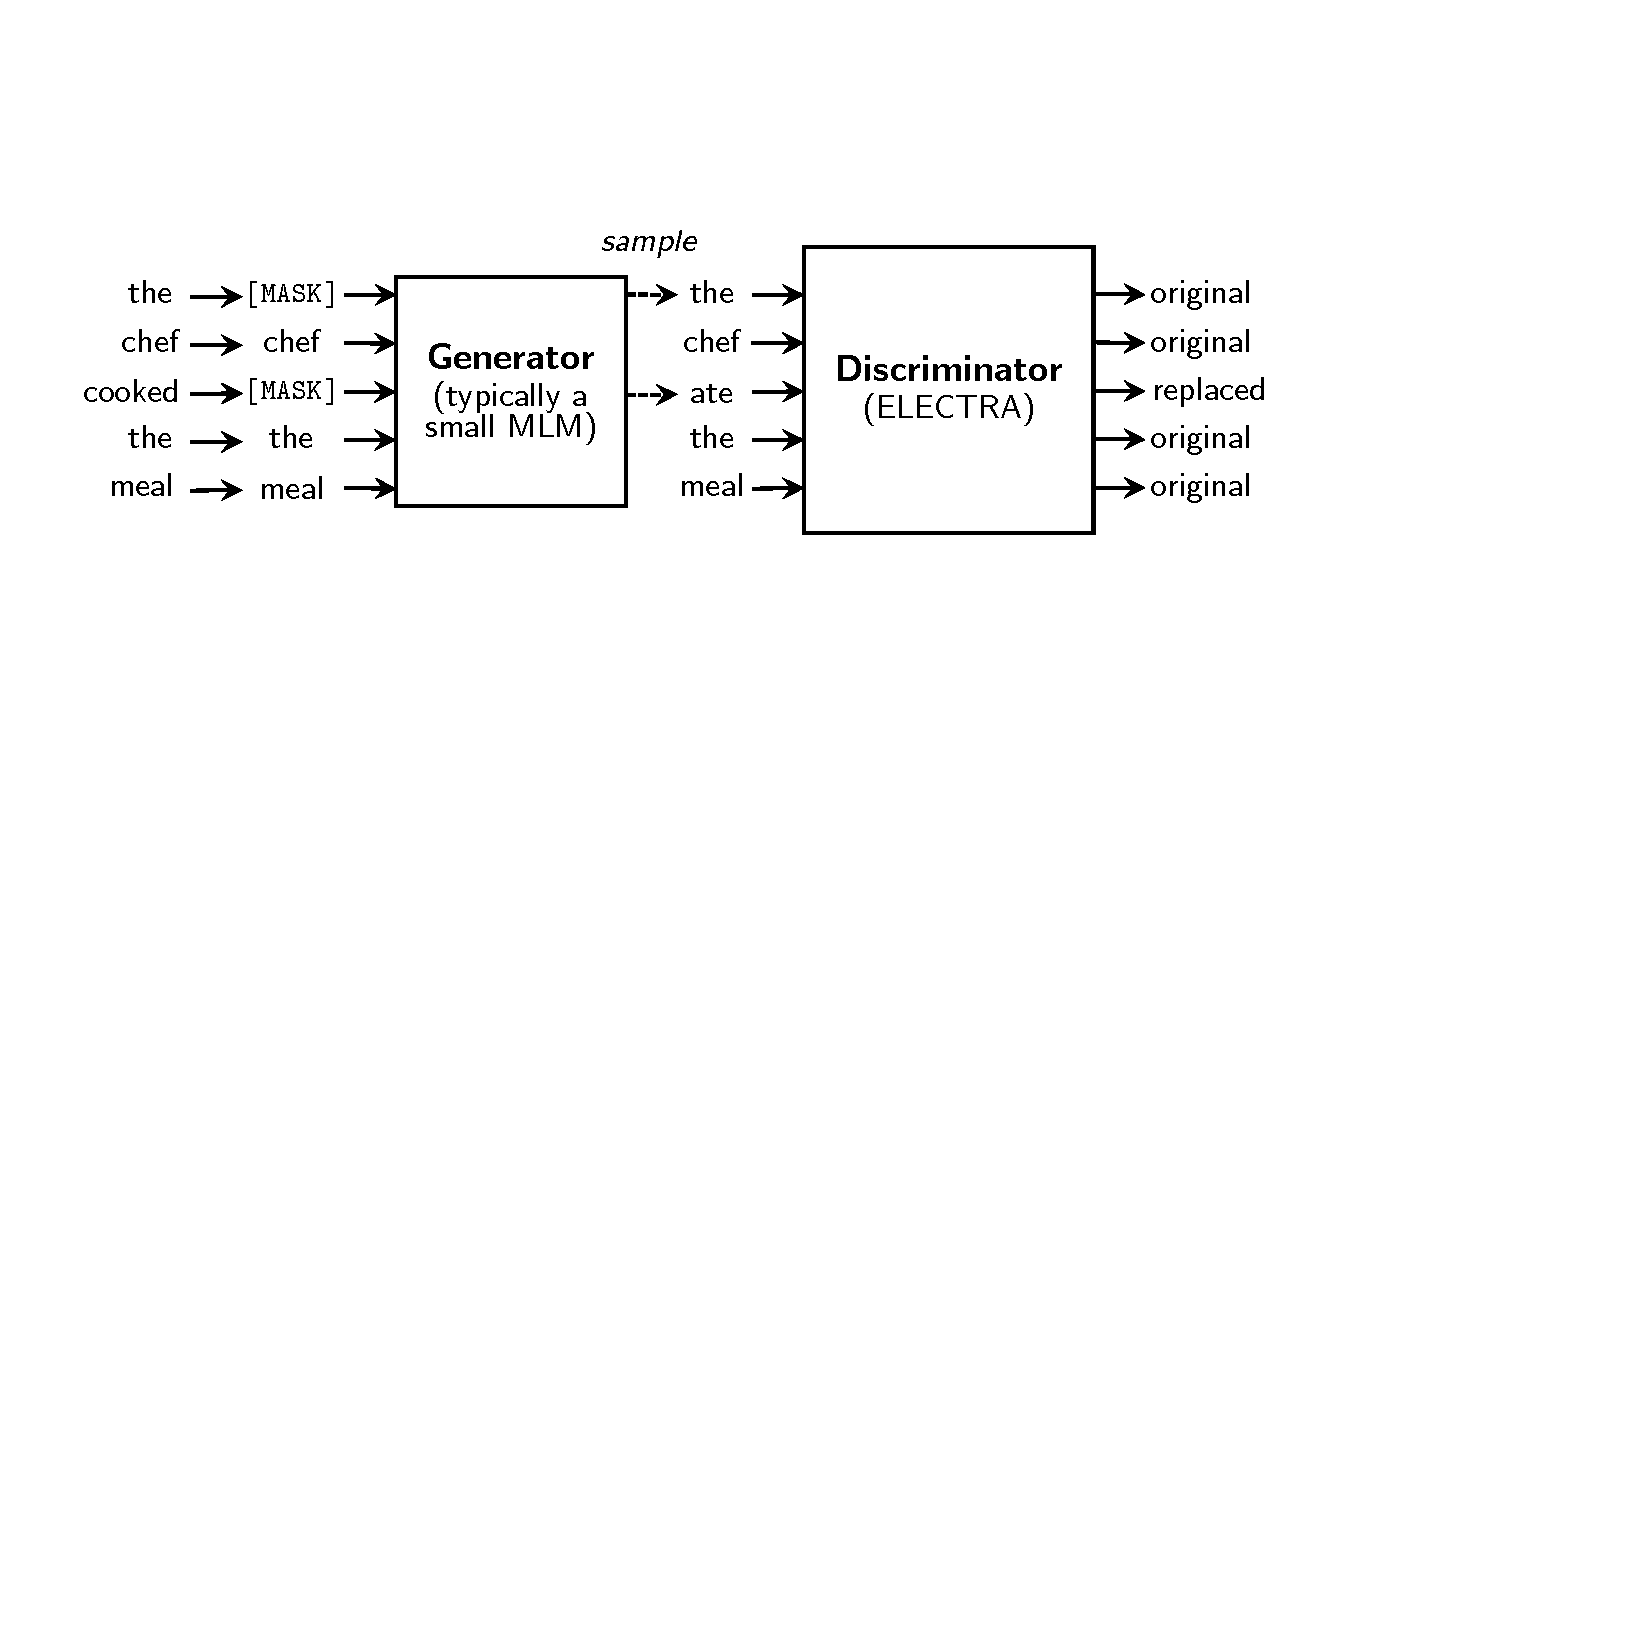
\includegraphics[width=0.9\textwidth]{figures/transfer_learning/electra.pdf}
  \caption{Illustration of ELECTRA model and the replaced token detection framework.}
  \label{fig:chp3_electra}
\end{figure*}

Specifically, as illustrated in \Cref{fig:chp3_electra}, the ELECTRA pre-training approach involves training a generator and a discriminator model simultaneously. The generator model is used to create corrupted versions of the input data by replacing some of the tokens with random tokens and is trained with the masked language modeling objective. The discriminator model is a larger and more complex model compared to the generator model and is trained to maximize the probability of correctly distinguishing between the original input data and the corrupted data at token level. After pre-training, the generator model is discarded and only the discriminator model is fine-tuned on downstream tasks. This training framework is more computationally efficient because it provides meaningful training signal on each input token, instead of only 15\% of the tokens that are masked. Experiments show that ELECTRA achieves competitive performance compared to the RoBERTa model with fewer computational budget.

\section{GPTs}

We then describe another important type of pre-trained language models, i.e., Transformer decoder models. These kind of models are \emph{true} language models according to the definition and can be used for generative tasks. The most representative models in this type are the GPT family pre-trained by OpenAI. We will introduce them as follows.

\paragraph{GPT.}

\begin{figure*}[t!]
  \centering
    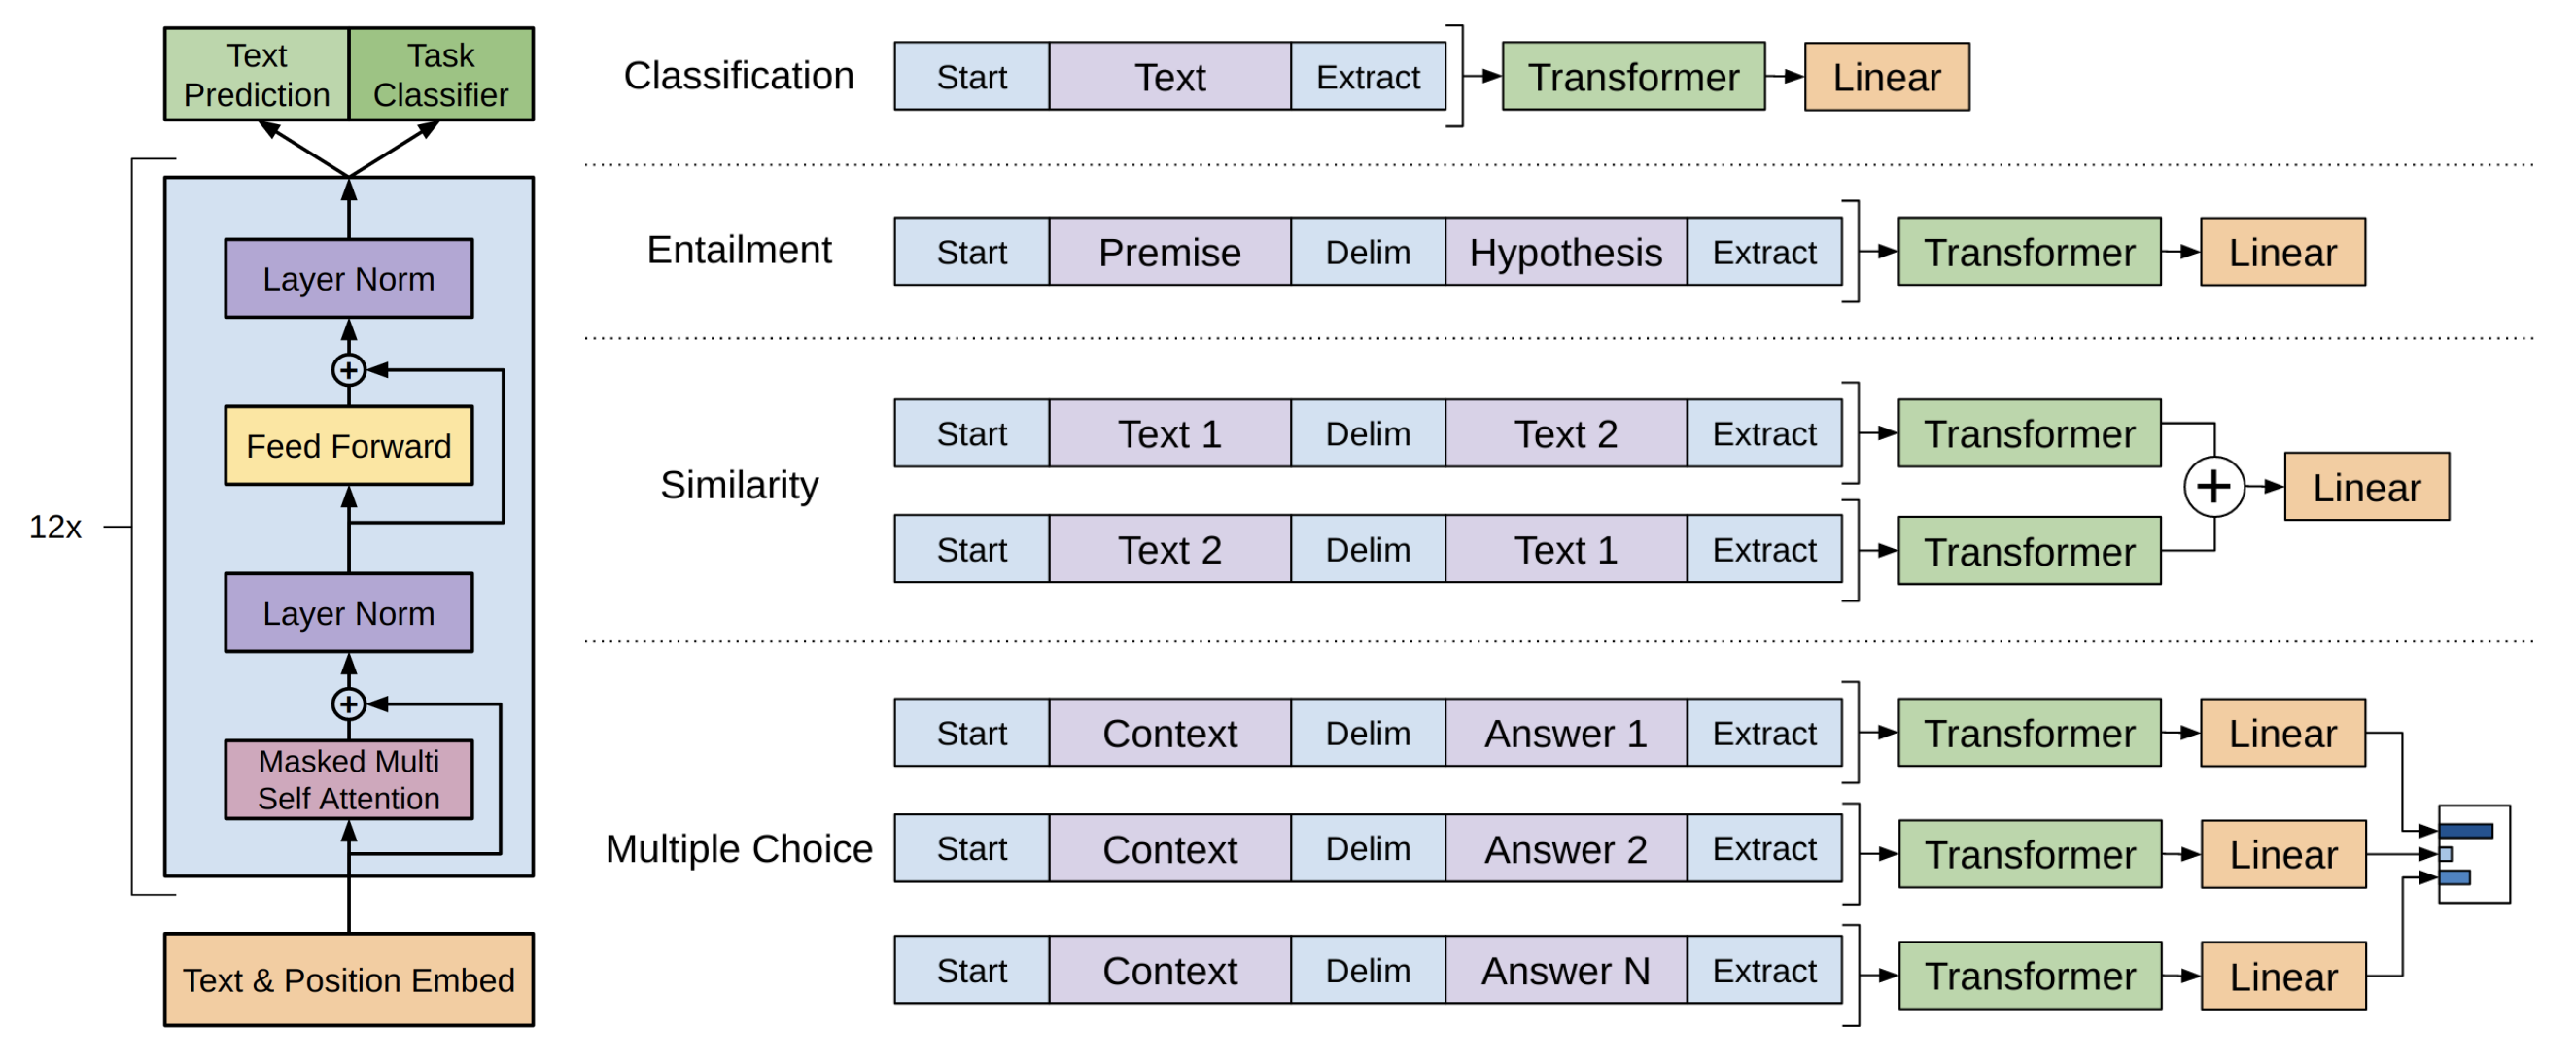
\includegraphics[width=\textwidth]{figures/transfer_learning/gpt.png}
  \caption{Illustration of how to fine-tune GPT on natural language understanding tasks. \TODO{take PDF screenshot}}
  \label{fig:chp3_gpt}
  \vspace{-3mm}
\end{figure*}

A few months before BERT is released, \citet{radford2018improving} pre-trained the first version of the GPT (Generative Pre-training Transformers) family. GPT is a decoder-only Transformer language model pre-trained with the standard language modeling objective on large scale web text. After pre-training, GPT can be fine-tuned on various natural language understanding tasks by transforming the inputs into a single text sequence. The sequence is fed into the GPT model and the final hidden state is used as the sequence representation, which is then fed into a fully-connected layer to produce predictions. The GPT fine-tuning procedure is illustrated in \Cref{fig:chp3_gpt}.


\paragraph{GPT-2.}

\begin{figure*}[t!]
  \centering
    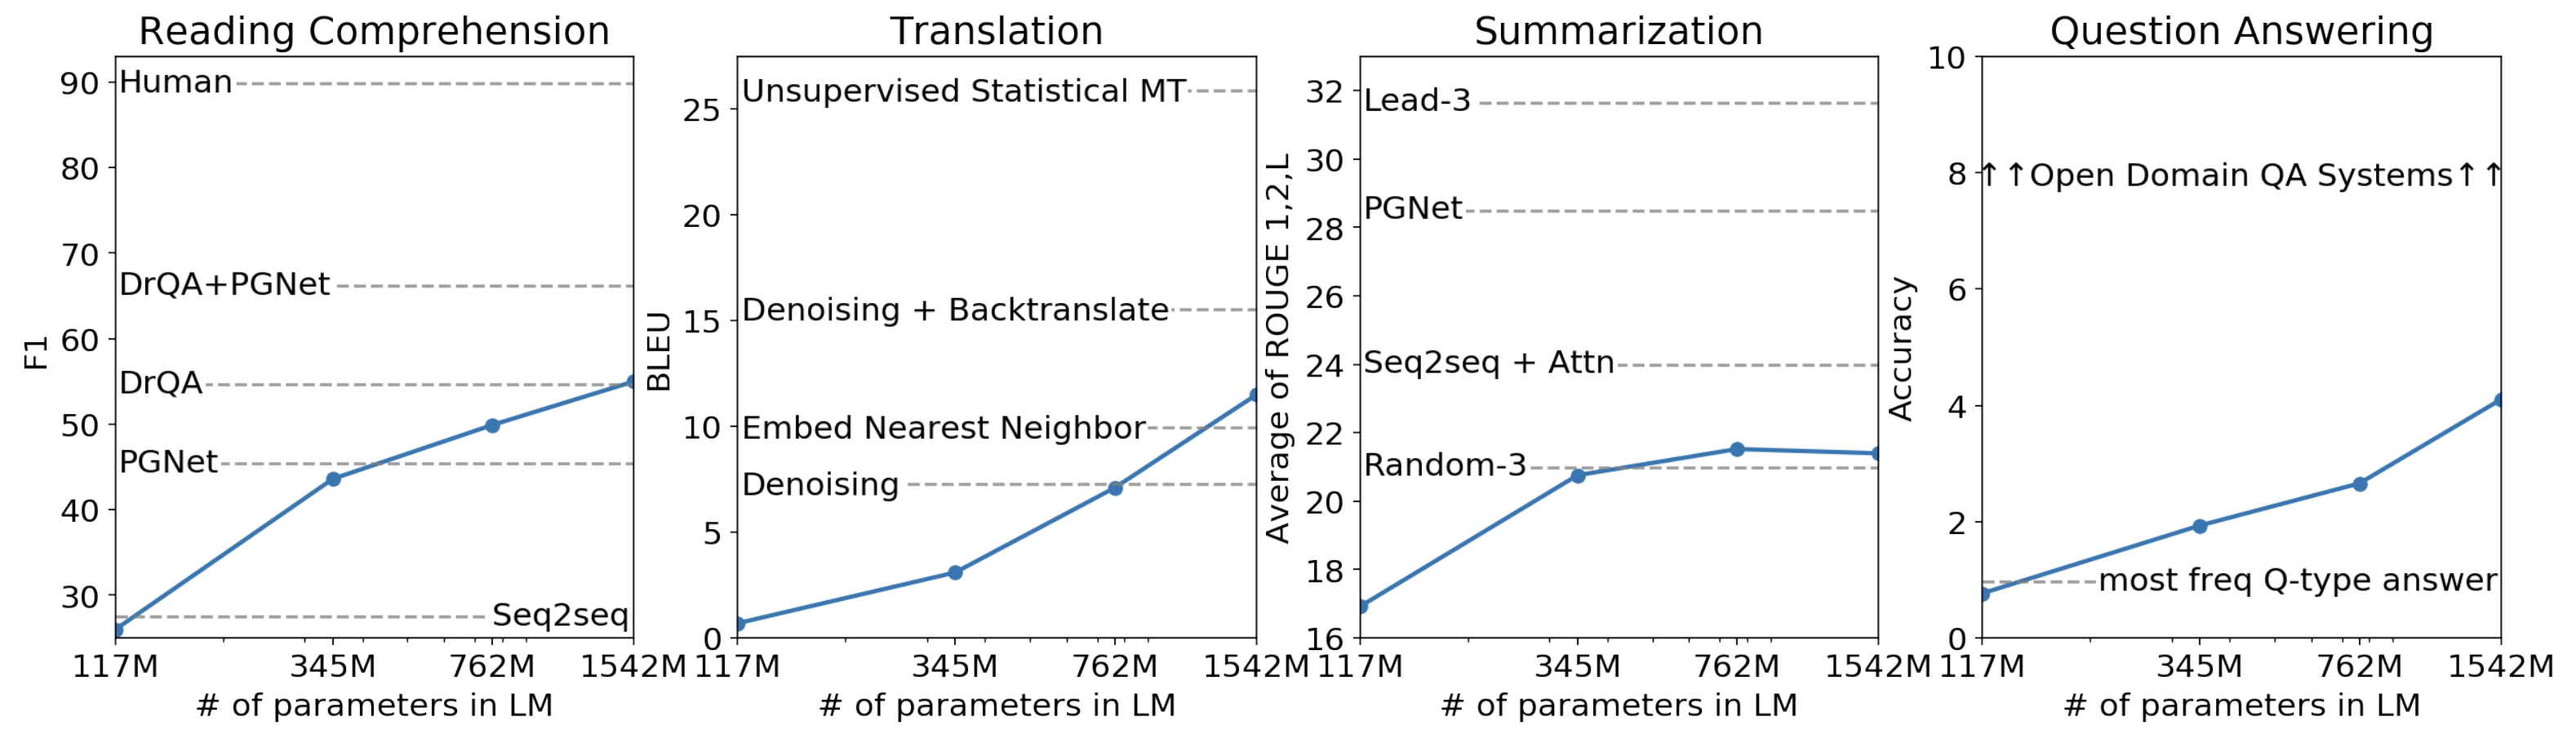
\includegraphics[width=\textwidth]{figures/transfer_learning/gpt2.png}
  \caption{Illustration of GPT-2's zero-shot performance on various NLP tasks with respect to model sizes. }
  % \TODO{take PDF screenshot}
  \label{fig:chp3_gpt2}
  \vspace{-1mm}
\end{figure*}

After the success of GPT, OpenAI further scales generative pre-training with GPT-2~\citep{radford2019language} with larger models and more training data. In addition to better performance with fine-tuning, they also find that generative pre-training on large scale text data makes the model becomes unsupervised multi-task learners that performs reasonably on various NLP tasks in the zero-shot setting. As shown in \Cref{fig:chp3_gpt2}, the zero-shot performance of GPT-2 significantly improves when scaling the model size, and the largest GPT-2 model with 1.5 Billion parameters achieves non-trivial performance on some NLP tasks. This for the first time demonstrate the potential of scaling LLM pre-training for zero-shot inference.

\paragraph{GPT-3.}

\begin{figure*}[t!]
  \centering
    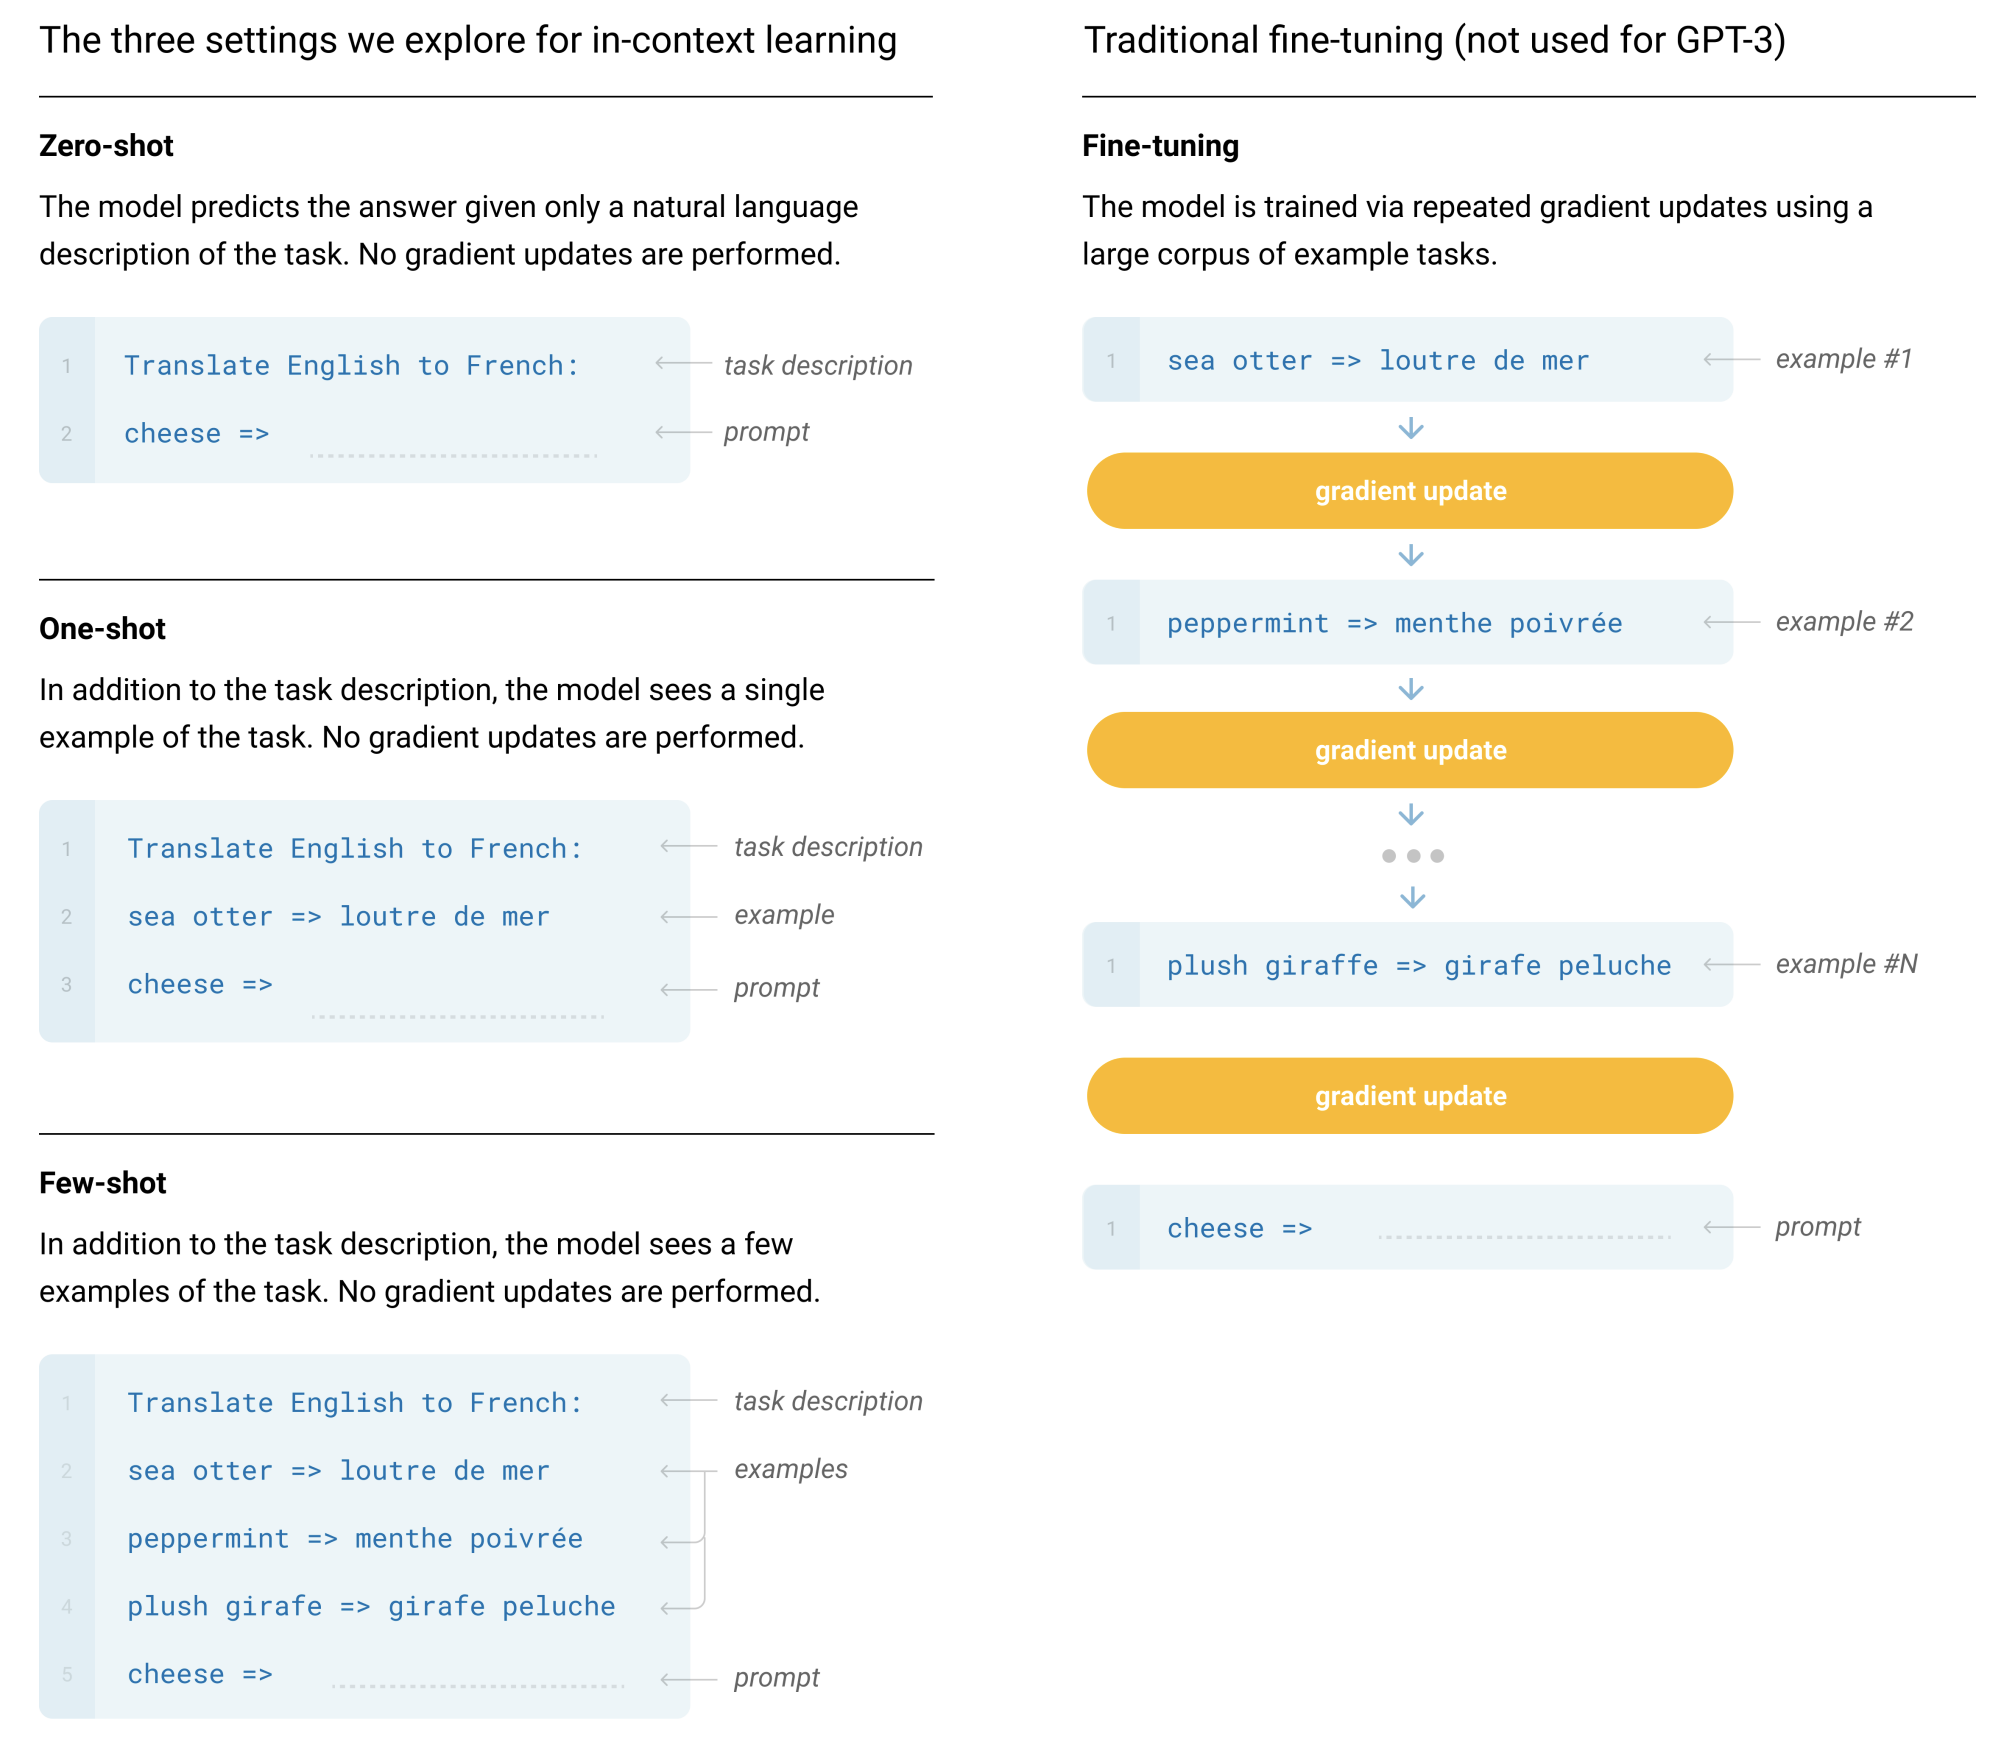
\includegraphics[width=\textwidth]{figures/transfer_learning/icl.png}
  \caption{Comparison of few-shot in-context learning with zero-shot learning and fine-tuning.}
  \label{fig:chp3_icl}
  \vspace{-3mm}
\end{figure*}


Motivated by the success of scaling model size and pre-training corpus in GPT-2, OpenAI further scales the size of decoder-only Transformer language models to 175 Billion, which is over 100 times larger compared to the largest GPT-2 model. They find that in addition to improved zero-shot performance, GPT-3 also exhibits strong few-shot ``in-context learning'' ability. As illustrated in \Cref{fig:chp3_icl}, in-context learning append both the task description and a few demonstrations of the task to the original input as the input for the language model, which produces the prediction by auto-regressively predicting next tokens. Different 

%\paragraph{ChatGPT?}

%\subsection{Multilingual LMs}
%\mrinmaya{Can we have a bit about mBERT and XLM-R too?}

\section{Seq2seq TLMs}

Apart from encoder-only and decoder-only Transformer language models, researchers also explored pre-training encoder-decoder Transformer language models. Compared to BERT-like encoder-only models and GPT-like decoder-only models, encoder-decoder models suits sequence-to-sequence generation tasks such as machine translation and text summarization better. This is because the encoder help the model better understand the input text with bidirectional attention flow, and the decoder help the model generate more fluent outputs. We will introduce T5~\citep{DBLP:journals/jmlr/RaffelSRLNMZLL20} and BART~\citep{DBLP:conf/acl/LewisLGGMLSZ20}, two representative pre-trained encoder-decoder Transformer language models, in this section.

\paragraph{T5.}

\begin{figure*}[t!]
  \centering
    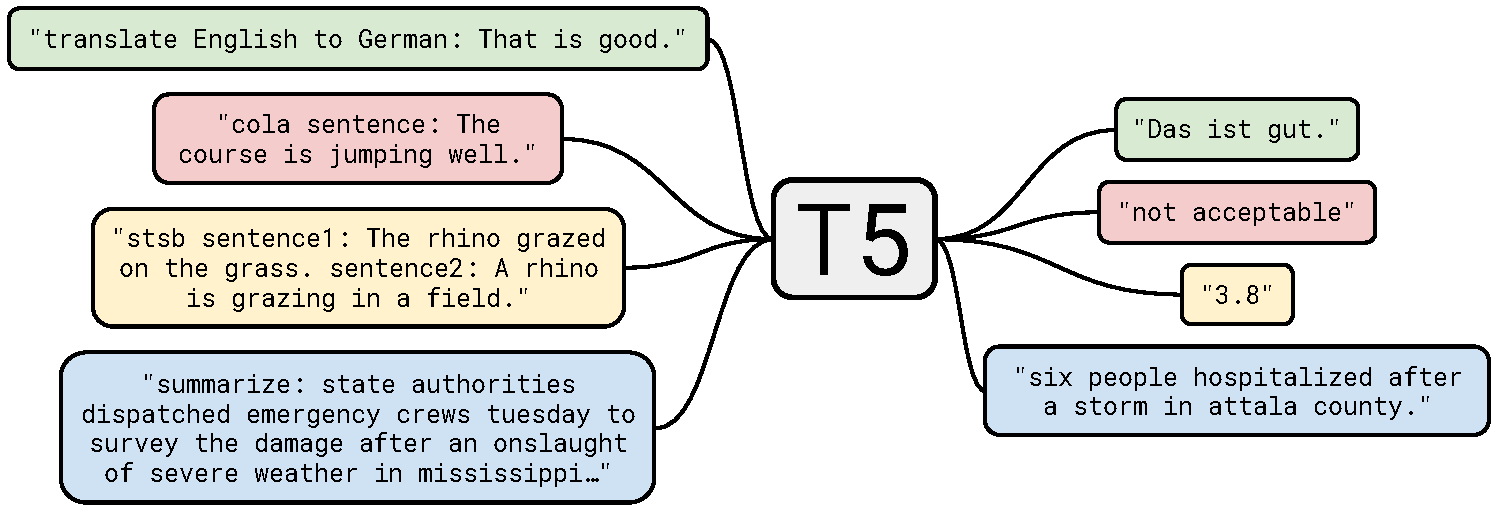
\includegraphics[width=\textwidth]{figures/transfer_learning/text_to_text.pdf}
  \caption{Illustration of the text-to-text framework of T5.}
  \label{fig:t5}
  \vspace{-3mm}
\end{figure*}

After the success of BERT and GPTs on natural language understanding and unconditional text generation, it is natural to consider pre-training an encoder-decoder model to improve seq2seq tasks. To this end, \citet{DBLP:journals/jmlr/RaffelSRLNMZLL20} pre-trained T5 (''Text-to-Text Transfer Transformer''), a powerful pre-trained encoder-decoder language model.

As illustrated in \Cref{fig:t5}, T5 is a general-purpose seq2seq model that can handle both natural language understanding and generation tasks with a text-to-text framework: the model take task description and task input as the encoder input and output the answer with the decoder. This paradigm is very influential to future NLP research because it demonstrates the possibility of building a single general-purpose model that can handle all NLP tasks.



\begin{figure*}[t!]
  \centering
  \begin{subfigure}[b]{0.49\textwidth}
    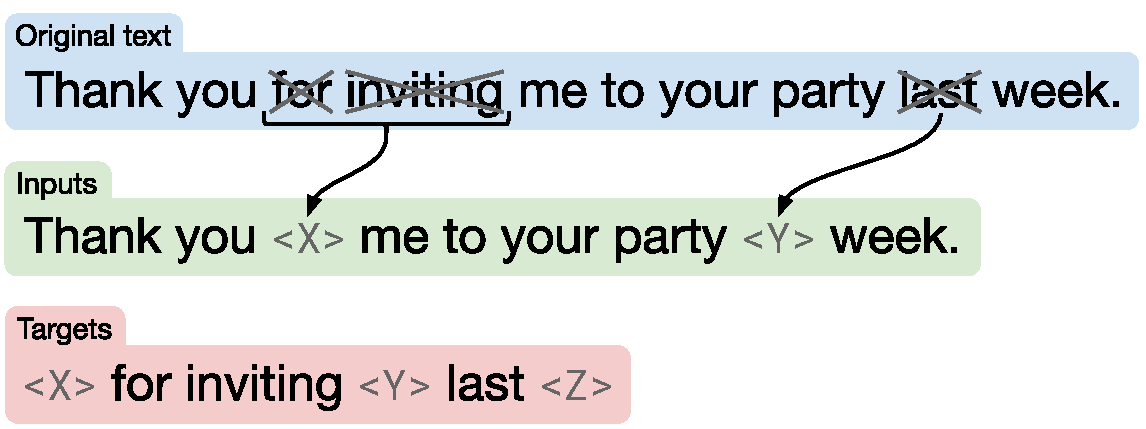
\includegraphics[width=\textwidth]{figures/transfer_learning/text_infilling.pdf}
    \caption{Text infilling objective.}
    \label{fig:text_infilling}
  \end{subfigure}
  \hfill
  \begin{subfigure}[b]{0.49\textwidth}
    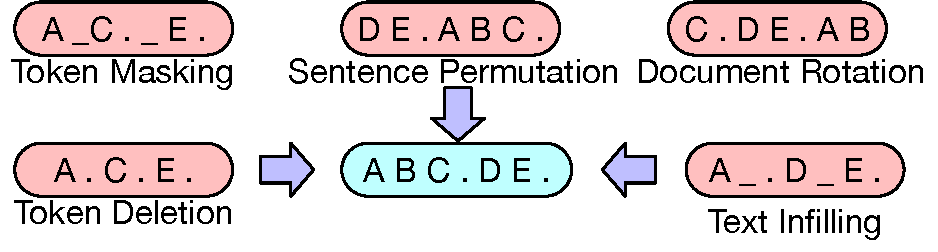
\includegraphics[width=\textwidth]{figures/transfer_learning/bart_noise.pdf}
    \caption{Noise functions investigated in BART pre-training.}
    \label{fig:bart_noise}
  \end{subfigure}
  \caption{Illustrations of the text infilling objective in T5 and other noise functions investigated in BART.}
  \label{fig:text_and_noise}
\end{figure*}
% \begin{figure*}[t!]
%   \centering
%     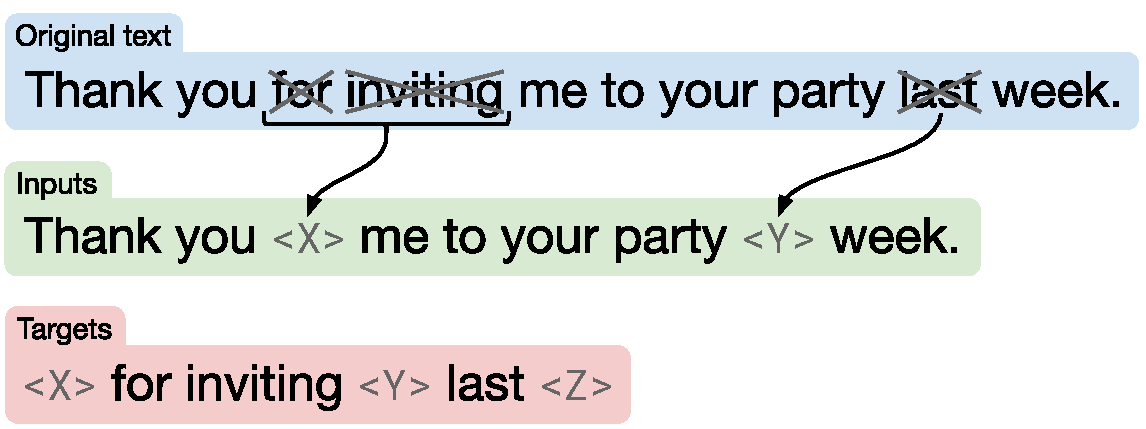
\includegraphics[width=\textwidth]{figures/transfer_learning/text_infilling.pdf}
%   \caption{Illustration of the text infilling objective.}
%   \label{fig:text_infilling}
%   \vspace{-3mm}
% \end{figure*}

% \begin{figure*}[t!]
%   \centering
%     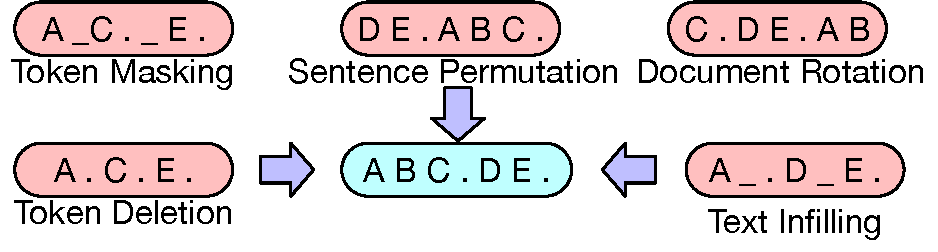
\includegraphics[width=\textwidth]{figures/transfer_learning/bart_noise.pdf}
%   \caption{Illustration of the noise functions investigated in BART pre-training.}
%   \label{fig:bart_noise}
%   \vspace{-3mm}
% \end{figure*}

T5 is pre-trained by mixing self-supervised data with multi-task supervised data. T5 uses a ``text infilling'' objective, which is shown to outperform other possible variants, as the source of self-supervision. As illustrated in \Cref{fig:text_infilling}, it randomly masks a portion of contiguous tokens and train the model to predict the masked text spans. \citet{DBLP:journals/jmlr/RaffelSRLNMZLL20} collected the C4 (''Colossal Clean Crawled Corpus'') dataset and construct massive text infilling data with it.  For supervised data, T5 convert training data for GLUE, SuperGLUE, machine translation, text summarization, question answering, etc., into text-to-text format by prepending task-specific prefixes. During pre-training, T5 randomly samples text-to-text training data according to the size of different tasks.

After pre-training, T5 can achieve competitive performance on supervised pre-training tasks without fine-tuning by prepending the corresponding prefix to the input. T5 also achieves state-of-the-art performance on a wide range of NLP tasks with task-specific fine-tuning.

\paragraph{BART.}

Concurrently with T5, \citet{DBLP:conf/acl/LewisLGGMLSZ20} pre-trained BART, another powerful seq2seq pre-trained model. As illustrated in \Cref{fig:bart_noise}, they investigated a number of noise functions as sources for self-supervision, and found the combination of text infilling and sentence permutation to be the best. Then it pre-trained BART on the same pre-training data as RoBERTa and obtained state-of-the-art performance on some natural language generation tasks. 
